\section{Adoracja Krzyża}
    
    \begin{itemize}
        \item po modlitwach \ii~ z \cc1 i \cc2 udają się krótką drogą do sedilii, gdzie \ii~ zdejmuje kapę - asystują \cc1 i \cc2
        \item formuje się procesja w kolejności:

        \begin{enumerate}\centering
            \item[] (stopnie ołtarza)
            \item[] \cc2~~~\ii~~~~\cc1
            \item[] \aa2~~~\aa1
        \end{enumerate}
    
        \item uczestniczący w procesji skłaniają się w stronę ołtarza i przechodzą do zakrystii krótką drogą
     
        \item z zakrystii rusza procesja w kolejności:
      
        \begin{enumerate}\centering
            \item[] \cc2~~~\cc1
            \item[] \aa2~~~\ii~~~~\aa1 
            \item[] 
            \item[] gdzie \aa~ trzymają świece, \ii~ - krzyż
        \end{enumerate}
    
        \item procesja długą drogą zmierza stopni ołtarza; po dojściu staje na posadzce po stronie epistoły
     
        \begin{figure}[h]
            \centering
            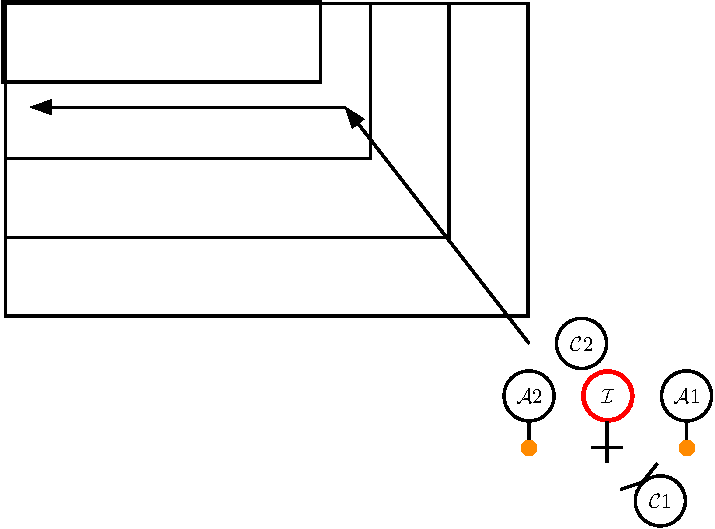
\includegraphics[scale=0.7]{Piatek/Obraz.pdf}
        \end{figure}
     
        \item \ii~ odsłaniając krzyż, śpiewa: \textit{Ecce lignum crucis}, na co wszyscy odpowiadając: \textit{Venite, adoremus} i klękają (ten schemat powtarza się w sumie 3-krotnie)
        \item \aa1 i \aa2 zostawiają akolitki po obu stronach krzyża, po czym odbierają od \ii~ krzyż
        \item \aa2 przynosi poduszkę na stopnie ołtarza; \aa1 i \aa2 kładą na nią krzyż
        \item \cc1 i \aa2 schodzą razem z \ii~ do sedilii i wszyscy ściągają obuwie
      
        \item adoracja następuje w kolejności:
     
        \begin{enumerate}\centering
            \item[] \ii~
            \item[] \cc1
            \item[] \aa2
            \item[] ministranci (dopóki nie przyjdą \aa1 i \aa2)
            \item[] \aa1
            \item[] \aa2 
            \item[] reszta ministrantów
        \end{enumerate}
     
        \item krzyż adorowany będzie przez ministrantów pojedynczo w sposób następujący:
     
        \begin{enumerate}[leftmargin=1cm]
            \item pierwsze przyklęknięcie ma miejsce przy balaskach
            \item drugie - w połowie prezbiterium
            \item trzecie - przy stopniach ołatarza
            \item następuje klęknięcie i pocałunek krzyża
            \item po wstaniu, ministrant wstaje, robi krok w bok, przyklęka z ministrantem, który właśnie doszedł do krzyża  i udaje się na swoje miejsce
            \item wszystkie przyklęknięcia wykonuje się \textbf{w tym samym czasie}, co ministrant przed nami!
        \end{enumerate}
      
        \begin{figure}[h]
            \centering
            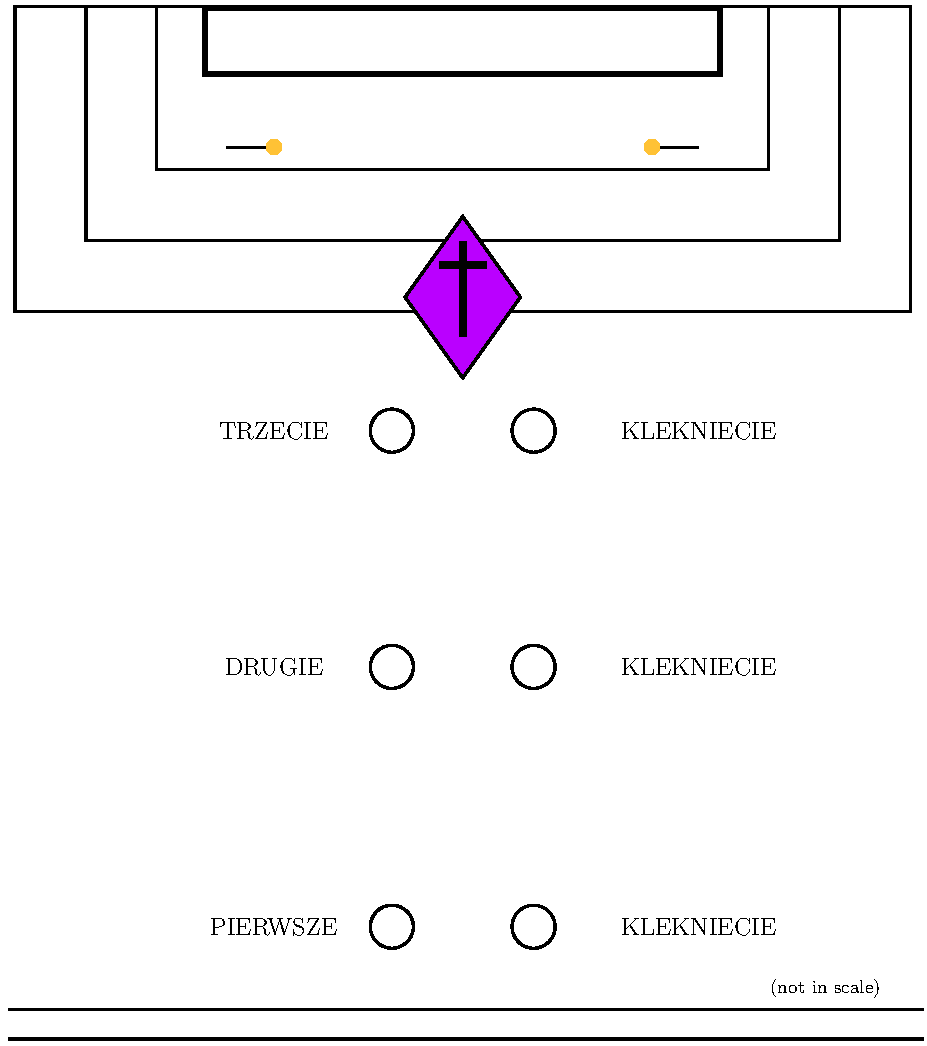
\includegraphics[scale=0.6]{Piatek/Adoracja.pdf}
        \end{figure}
     
        \item \cc1 i \aa2 po dokananiu adoracji, odbierają od \aa1 i \aa2 krzyż i go trzymają
        \item \aa1 i \aa2 po dokonaniu adoracji i nałożeniu butów, klękają po obu stronach krzyża twarzą do siebie na środkowym stopniu ołtarza przy akolitkach  
        \item po skończeniu adoracji przez ministrantów, \cc1 i \aa2 zanoszą krzyż przed prezbiterium w towarzystwie \aa1 i \aa2 ze świecami
        \item \aa1 i \aa2 stwaiają świece po bokach krzyża i odbierają od \cc1 i \aa2 krzyż i go trzymają
        \item po skończonej adoracji \cc1 i \aa2 odbierają od \aa1 i \aa2 krzyż i zanoszą go do stopni ołtarza
        \item tam dołącza do nich \ii~ i wszyscy trzej wchodzą po stopniach i \ii~ umieszcza krzyż na tabernakulum
        \item w międzyczasie \aa1 i \aa2 biorą swoje świece i stawiają je na ołtarzu
    \end{itemize}
    